% =============================================================================
% Neural Network Field Map Approximation for LHCb Track Extrapolation
% =============================================================================
\documentclass[11pt,a4paper]{article}

\usepackage[utf8]{inputenc}
\usepackage[T1]{fontenc}
\usepackage{amsmath,amssymb}
\usepackage{booktabs}
\usepackage{graphicx}
\usepackage{hyperref}
\usepackage[margin=2.5cm]{geometry}
\usepackage{xcolor}
\usepackage{caption}
\usepackage{subcaption}

\newcommand{\SI}[2]{#1\,#2}
\newcommand{\si}[1]{#1}

\title{Neural Network Approximation of the LHCb Magnetic Field Map\\
       for Fast Track Extrapolation}
\author{G.\ Scriven}
\date{\today}

\begin{document}
\maketitle

\begin{abstract}
    Track extrapolation through the LHCb dipole magnet requires repeated
    evaluation of a trilinear-interpolated magnetic field map---a
    memory-bound operation that dominates the cost of Runge--Kutta-based
    extrapolators.  We investigate replacing the field-map lookup with a
    small neural network that maps spatial coordinates
    $(x,y,z) \to (B_x,B_y,B_z)$.  A first generation of 30~models,
    spanning five widths, three depths, and two activations, achieved
    mean absolute errors as low as 0.5\,G but suffered from
    catastrophic failure in strong-field regions: relative errors
    exceeding 99\% where
    $|\mathbf{B}| > 100$\,G.  Analysis reveals that the extreme
    class imbalance of the field distribution---89.6\% of the grid volume
    has $|\mathbf{B}| < \SI{1}{G}$---causes standard MSE training to
    collapse the network toward zero output.  This motivates a second
    generation of experiments comparing eight loss functions and
    curriculum-learning schedules designed to correct this failure mode.
\end{abstract}

\tableofcontents
\newpage

% ─────────────────────────────────────────────────────────────────────────────
\section{Motivation}
\label{sec:motivation}
% ─────────────────────────────────────────────────────────────────────────────

\subsection{Track extrapolation in LHCb}

The LHCb experiment at the Large Hadron Collider reconstructs the
trajectories of charged particles produced in proton--proton collisions.
A central task in the reconstruction software is \emph{track
extrapolation}: propagating the five-parameter track state
$(x, y, t_x, t_y, q/p)$ from one $z$-plane to another through the
magnetic field of the dipole magnet.  Multiple extrapolation algorithms
are implemented in the \texttt{Rec} stack, the most physics-accurate
being the fourth-order Runge--Kutta (RK4) extrapolator
(\texttt{TrackRungeKuttaExtrapolator}).

Each RK4 step requires four evaluations of the magnetic field
$\mathbf{B}(x,y,z)$; a typical track traversing the full magnet
($z \in [200, 9500]\;\text{mm}$) uses on the order of
40 field evaluations.  High-level trigger (HLT) processing at
\SI{30}{MHz} crossing rate makes extrapolation a significant fraction
of the total CPU budget, and any factor-of-two speedup would be
directly beneficial to physics throughput.

\subsection{The field-map lookup bottleneck}

The LHCb magnetic field is stored as a regular 3D grid of
$81 \times 81 \times 146 = 957{,}906$ vertices spanning
\begin{align}
    x &\in [-4000, 4000] \;\text{mm}, \quad \Delta x = \SI{100}{mm}, \nonumber \\
    y &\in [-4000, 4000] \;\text{mm}, \quad \Delta y = \SI{100}{mm}, \\
    z &\in [-500, 14000]  \;\text{mm}, \quad \Delta z = \SI{100}{mm}. \nonumber
\end{align}
Each vertex stores the three components $(B_x, B_y, B_z)$ in Gauss.
At query time, trilinear interpolation is performed over the eight
surrounding grid corners, requiring eight loads from a
$957{,}906 \times 3 \times 8 = \SI{23}{MB}$ look-up table (single
precision).  This data structure far exceeds the L1 cache
(\SI{32}{KB}) of modern CPUs, making each field evaluation a
cache-miss-dominated, memory-bound operation.

\subsection{Replacing the field map with a neural network}

The key observation is that the field map is a smooth, deterministic
function $\mathbf{B}: \mathbb{R}^3 \to \mathbb{R}^3$.  A small
feedforward network (MLP) with $\mathcal{O}(200\text{--}20{,}000)$
parameters would fit entirely in L1 cache and replace every trilinear
interpolation with a sequence of fused multiply-add operations---a
compute-bound workload that modern CPUs handle efficiently.

The extrapolation algorithm itself (RK4, Cash--Karp, parabolic, etc.)
remains unchanged; only the field evaluation is substituted.  This is
the minimal-invasiveness approach: no retraining of the integrator, no
change to the track model, and a single header file
(\texttt{FieldMapNNWeights.h}) encapsulates the entire replacement.

The equations of motion for a charged particle in a magnetic field are
\begin{equation}
    \frac{d\mathbf{r}}{dz} = \begin{pmatrix} t_x \\ t_y \\ 1 \end{pmatrix},
    \qquad
    \frac{dt_x}{dz} = \frac{q}{p}\,n\bigl(
        t_y(t_x B_x + B_z) - (1+t_x^2)\,B_y
    \bigr),
    \label{eq:lorentz}
\end{equation}
with an analogous expression for $dt_y/dz$, where
$n = c\sqrt{1 + t_x^2 + t_y^2}$ is a normalisation factor and $c$ is the
speed of light.  The field components $B_x$, $B_y$, $B_z$ enter
linearly, so any proportional error in the field translates directly
into a proportional error in the computed deflection.  The
\emph{relative} accuracy of the field approximation is therefore the
physically meaningful metric, not the mean absolute error.

\subsection{Computational cost breakdown}
\label{sec:cost}

To quantify the potential speedup, we performed native C++
micro-benchmarks of every sub-component of a Cash--Karp track
extrapolation (see companion document
\texttt{extrapolator\_cost\_analysis.pdf} for full details).  All
timings use \texttt{std::chrono::high\_resolution\_clock} with
100{,}000 iterations on an AMD EPYC~7551P, compiled at
\texttt{-O2~-march=native}.

\paragraph{Key measured timings.}
\begin{center}
\begin{tabular}{lrl}
\toprule
Component & Time (ns) & Notes \\
\midrule
Trilinear interpolation & 100 & 8~loads from 23\,MB grid \\
NN~[32] SiLU (227 params) & 872 & $8.8\times$ slower (32 \texttt{exp()} calls)\\
Lorentz derivative & 14 & 14~FLOPs + 1 \texttt{sqrt} \\
Cash--Karp step (trilinear) & 385 & 6 field + 6 deriv + bookkeeping \\
Full track, 10 steps (trilinear) & 2625 & $\approx 2.50\;\mu$s production \\
Full track, 10 steps (NN~[32]) & 30{,}269 & $11.5\times$ \emph{slower} \\
\bottomrule
\end{tabular}
\end{center}

\paragraph{FLOP decomposition.}
A single Cash--Karp step comprises 558~FLOPs:
B-field lookup accounts for 60\% (336~FLOPs),
the Lorentz derivative for 18\% (102~FLOPs),
and Butcher-tableau bookkeeping for 22\% (120~FLOPs).

\paragraph{Two speedup strategies.}
\textbf{Strategy~A} (replace only the field lookup) is bounded by
Amdahl's law with $f = 0.60$ and a maximum speedup of $2.5\times$.
However, the NN~[32] SiLU is $8.8\times$ \emph{slower} per call than
trilinear, making Strategy~A non-viable with current activations:
the measured full-track slowdown is $11.5\times$.
\textbf{Strategy~B} (replace the entire extrapolator with a single NN
forward pass) eliminates all 60~field evaluations and is estimated at
$\sim$\SI{2.0}{\textmu s}---a $1.3\times$ speedup over the
\SI{2.5}{\textmu s} production baseline.

\begin{figure}[htbp]
\centering
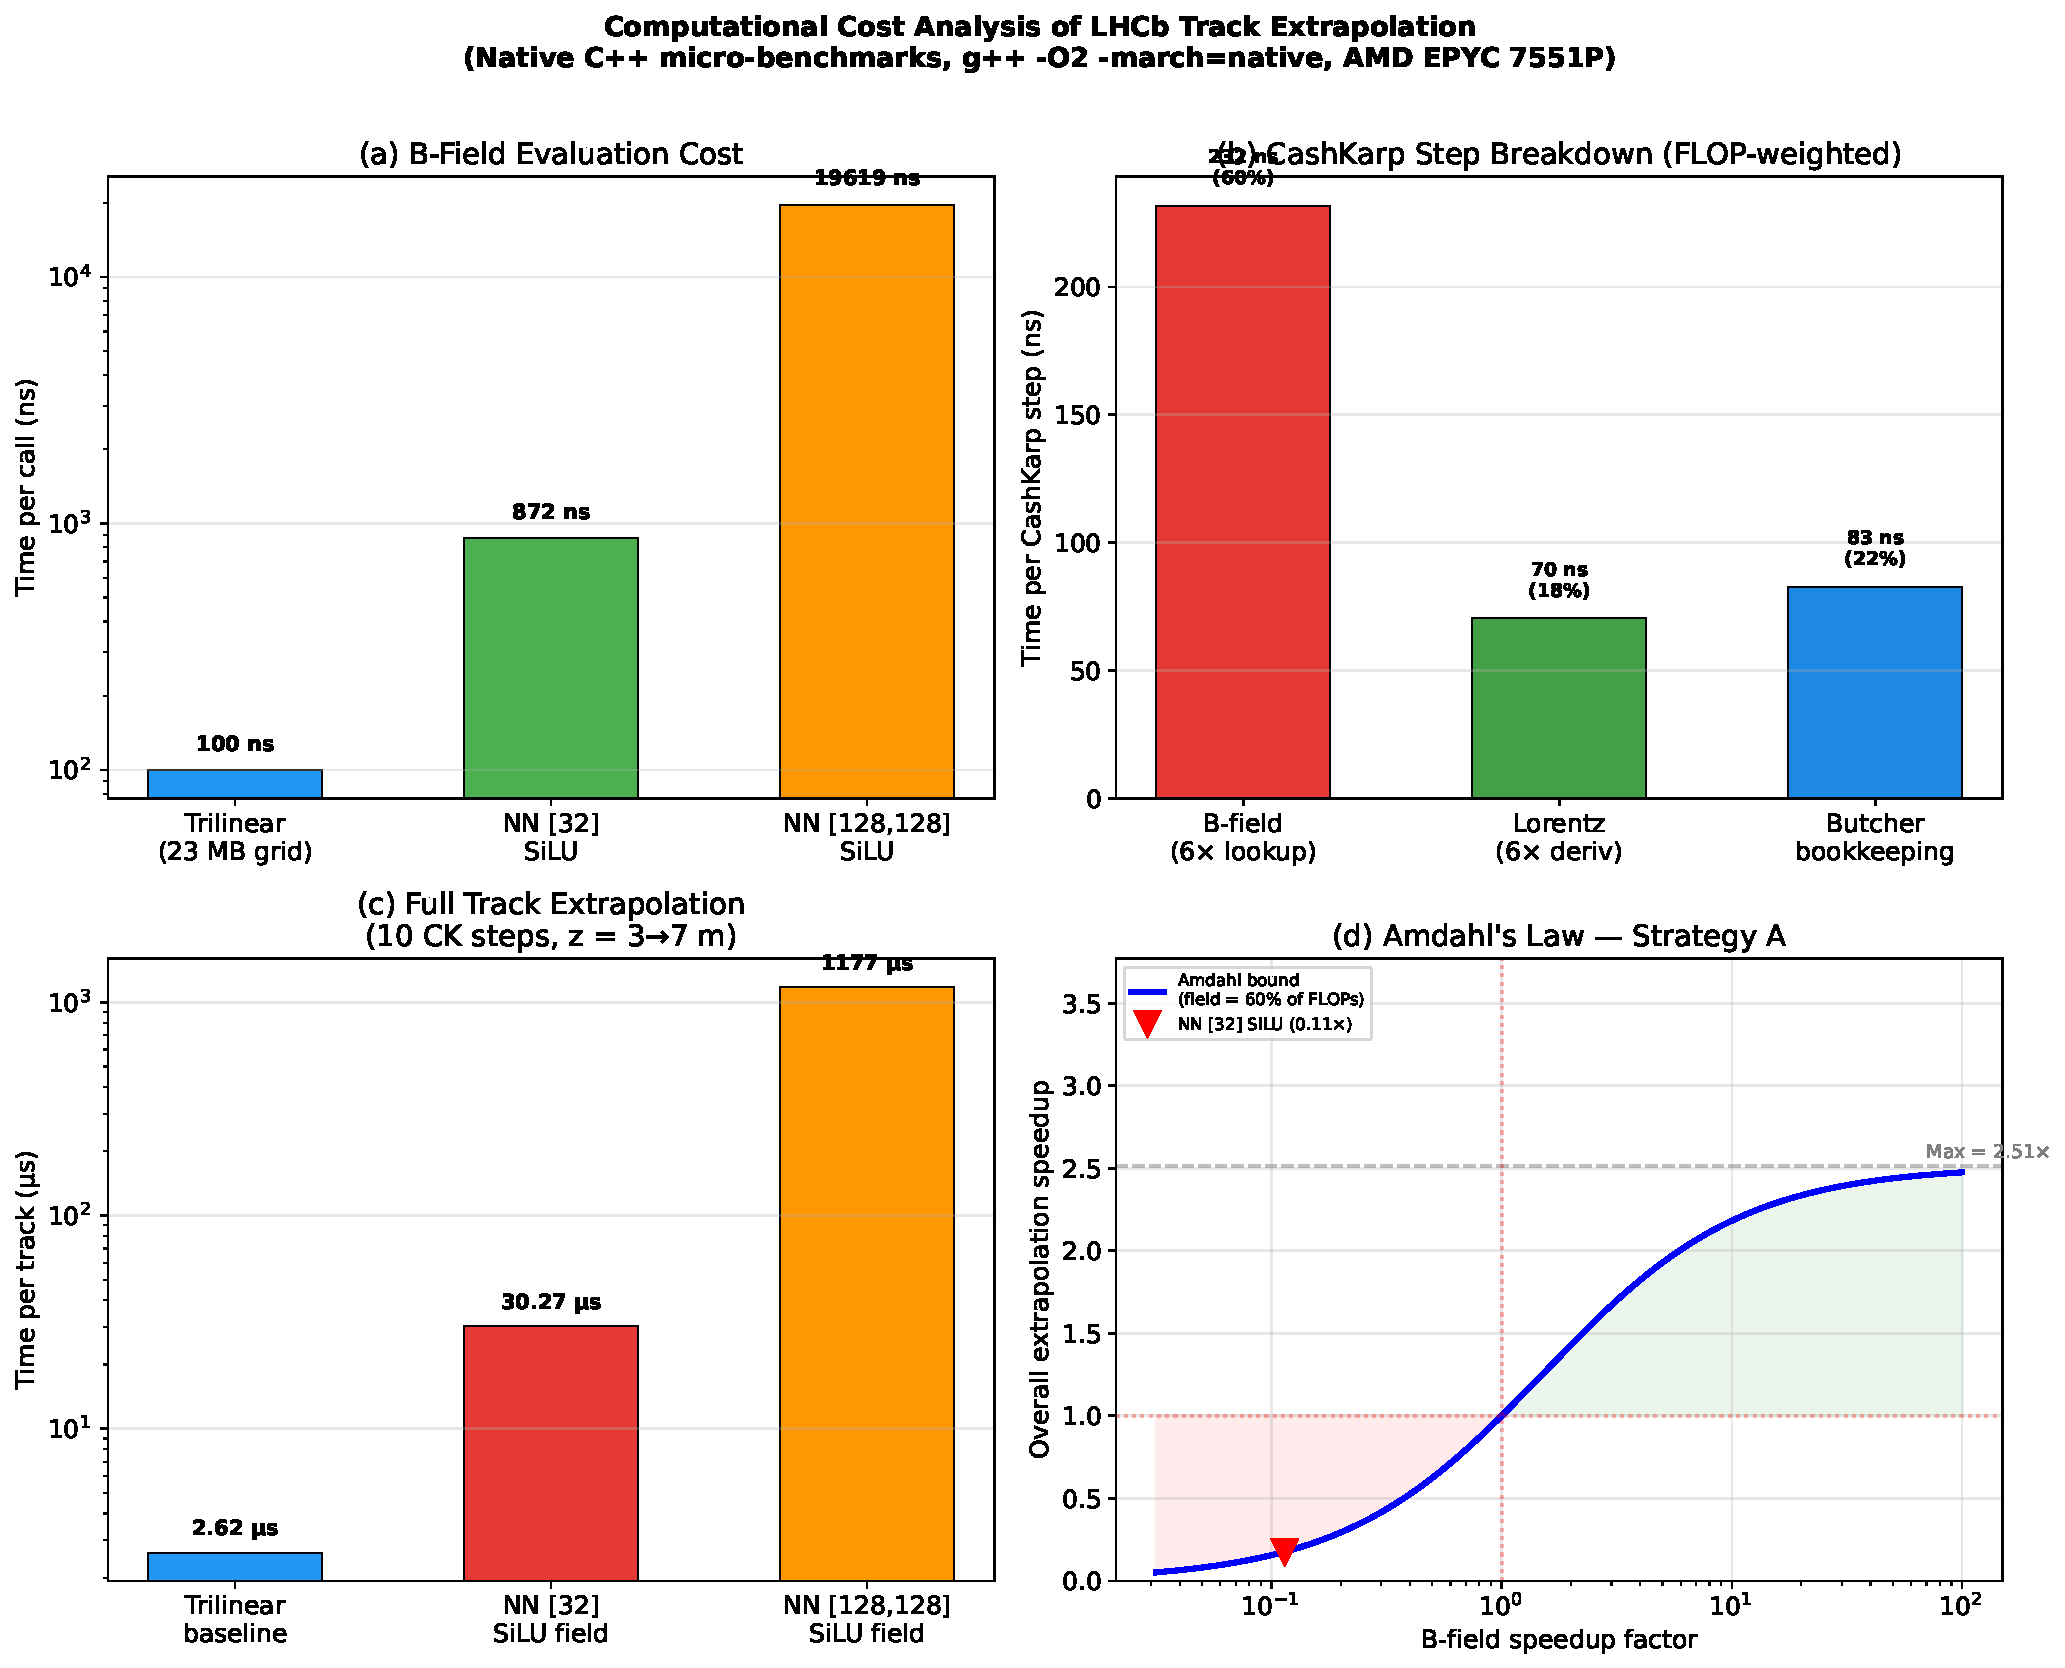
\includegraphics[width=\textwidth]{plots/cost_analysis_summary.pdf}
\caption{Computational cost breakdown of LHCb track extrapolation from
native C++ micro-benchmarks.  (a)~Per-call B-field evaluation cost.
(b)~FLOP-weighted Cash--Karp step decomposition.  (c)~Full track timing
with different field methods. (d)~Amdahl's law bound for Strategy~A,
showing the NN~[32] SiLU operating point deep in the ``slower'' regime.}
\label{fig:cost_summary}
\end{figure}

These results motivate pursuing Strategy~B (full NN extrapolator) as
the primary path, while Strategy~A requires faster activations (ReLU)
or hardware acceleration to break even.  Nevertheless, an NN field map
with sufficient accuracy remains valuable for physics validation and as
a stepping stone toward a full NN extrapolator.

% ─────────────────────────────────────────────────────────────────────────────
\section{Generation~1: Architecture Grid Search}
\label{sec:gen1}
% ─────────────────────────────────────────────────────────────────────────────

\subsection{Experimental setup}

A grid search was conducted over 30~network architectures, defined by
the Cartesian product of:
\begin{itemize}
    \item \textbf{Width}: $\{32, 64, 128, 256, 512\}$ hidden units per layer,
    \item \textbf{Depth}: $\{1, 2, 3\}$ hidden layers,
    \item \textbf{Activation}: $\{\text{ReLU}, \text{SiLU}\}$.
\end{itemize}
All models share the same \texttt{FieldMLP} architecture: a Sequential
stack of \texttt{Linear}$+$activation layers with a 3-dimensional input
$(x,y,z)$ and 3-dimensional output $(B_x, B_y, B_z)$.  Inputs and
outputs are independently standardised (zero mean, unit variance).

Training used all 957{,}906 grid vertices as training data and
100{,}000 random off-grid points (with trilinear-interpolated ground
truth) for validation.  The loss function was the standard mean squared
error (MSE) on the normalised targets:
\begin{equation}
    \mathcal{L}_{\text{MSE}} = \frac{1}{N}\sum_{i=1}^{N}
        \left\lVert \hat{\mathbf{y}}_i - \mathbf{y}_i \right\rVert^2,
    \label{eq:mse}
\end{equation}
where $\hat{\mathbf{y}}_i$ and $\mathbf{y}_i$ are the predicted and
true normalised field vectors.  Training ran for up to 200~epochs with
Adam (learning rate $10^{-3}$), cosine annealing, and early stopping
(patience = 20).

All 30~jobs were submitted to the Nikhef STBC HTCondor cluster with
one GPU per job.

\subsection{Results}

\begin{table}[t]
    \centering
    \caption{Summary of Generation~1 results.  MAE and maximum error are
    in Gauss.  SiLU consistently outperforms ReLU at every architecture.}
    \label{tab:gen1_summary}
    \begin{tabular}{llrrrr}
        \toprule
        Activation & Depth$\times$Width & Parameters & FLOPs &
        MAE (G) & Max error (G) \\
        \midrule
        SiLU & $3 \times 256$ & 133{,}379 & 268{,}288 & 0.50 & 14{,}675 \\
        SiLU & $2 \times 128$ &  17{,}411 &  35{,}328 & 0.70 & 16{,}988 \\
        SiLU & $1 \times 32$  &     227   &     512   & 0.82 & 16{,}814 \\
        ReLU & $2 \times 512$ & 266{,}243 & 531{,}456 & 0.60 & 17{,}398 \\
        ReLU & $1 \times 32$  &     227   &     320   & 1.02 & 16{,}995 \\
        \bottomrule
    \end{tabular}
\end{table}

Table~\ref{tab:gen1_summary} presents a subset of the 30~models.
The global MAE ranged from \SI{0.50}{G} (SiLU $3{\times}256$) to
\SI{1.15}{G} (ReLU $1{\times}32$), and SiLU was uniformly superior to
ReLU at every width and depth.

At first glance these errors appear excellent: a \SI{0.5}{G} MAE
against a peak field of \SI{33024}{G} (\SI{3.30}{T}) suggests a mean
relative error of $\sim 10^{-5}$.  However, inspection of the
\emph{maximum} error column reveals that every model has a maximum
error of approximately \SI{17000}{G}---roughly half the peak field
strength.  This maximum does not improve meaningfully with model
capacity: the 227-parameter model and the 133{,}379-parameter model
both show maximum errors of $\sim$\num{15000}--\num{17000}\;\text{G}.

\subsection{Failure analysis: the class-imbalance catastrophe}
\label{sec:failure}

The root cause is the extreme imbalance of the field magnitude
distribution over the grid volume.  Table~\ref{tab:field_dist} quantifies
this.

\begin{table}[h]
    \centering
    \caption{Distribution of $|\mathbf{B}|$ over the 957{,}906 field-map
    grid vertices.}
    \label{tab:field_dist}
    \begin{tabular}{lr}
        \toprule
        Region & Fraction of grid \\
        \midrule
        $|\mathbf{B}| < \SI{1}{G}$    & 89.6\% \\
        $|\mathbf{B}| < \SI{10}{G}$   & 99.0\% \\
        $|\mathbf{B}| > \SI{100}{G}$  &  0.1\% \\
        $|\mathbf{B}| > \SI{1000}{G}$ & $<0.1\%$ \\
        \bottomrule
    \end{tabular}
\end{table}

The LHCb dipole field is concentrated in a narrow cylindrical core
around the beam axis near $z \approx \SI{5000}{mm}$, while the vast
majority of the grid volume is in field-free regions upstream,
downstream, and off-axis.  With MSE training
(Eq.~\ref{eq:mse}), a sample at $|\mathbf{B}| = \SI{1}{G}$ and a sample
at $|\mathbf{B}| = \SI{33000}{G}$ contribute equally to the loss if
both have the same \emph{absolute} residual.  Since 99\% of samples
have $|\mathbf{B}| < \SI{10}{G}$, the optimal strategy under uniform
MSE is to predict approximately zero everywhere.  This explains why:

\begin{enumerate}
    \item The \emph{global} MAE is dominated by the 89.6\% of points
          with near-zero field, producing a deceptively low value
          ($\sim$\SI{0.5}{G}).
    \item The \emph{maximum} error is approximately equal to the peak
          field ($\sim$\SI{17000}{G}), because the network has learned
          to output $\approx 0$ even in the magnet core.
    \item Increasing model capacity (from 227 to 133{,}379 parameters)
          does not help, because the loss landscape itself provides no
          gradient signal to learn the strong-field region.
\end{enumerate}

We verified this diagnosis by computing relative errors at specific
high-field points.  At the field maximum
$(x, y, z) = (0, -3900, 5000)\;\text{mm}$, where the true field is
$B_y = -\SI{33024}{G}$, the best-MAE model (SiLU $3{\times}256$)
predicts $B_y \approx -\SI{1936}{G}$---a relative error of 94\%.  The
speed-viable model (SiLU $1{\times}32$) predicts
$B_y \approx \SI{3}{G}$---a relative error of $>99.99\%$.

These errors propagate directly through Eq.~\ref{eq:lorentz}: a track at
\SI{1}{GeV/c} momentum extrapolated from $z = 200$ to
$\SI{9500}{mm}$ using the NN field (viable model) arrives with a
position offset of \SI{1503}{mm} and a slope error of 0.33 compared to the trilinear
reference.  The NN field map is, in its current form, physically
unusable.

% ─────────────────────────────────────────────────────────────────────────────
\section{Generation~2: Loss Function and Training Strategy Comparison}
\label{sec:gen2}
% ─────────────────────────────────────────────────────────────────────────────

\subsection{Motivation}

The Generation~1 failure is not a capacity problem but a
\emph{loss-function} problem.  The field distribution spans five
orders of magnitude ($\sim$\SI{0.01}{G} to $\sim$\SI{33000}{G}), and
any loss that treats all residuals equally will be dominated by the
99\% of near-zero samples.  To fix this, the loss must either:
\begin{enumerate}
    \item[(a)] \textbf{Re-weight} samples so that the rare high-field
               points contribute proportionally more to the gradient;
    \item[(b)] \textbf{Transform} the targets into a space where the
               dynamic range is compressed (e.g.\ logarithmic); or
    \item[(c)] Use a \textbf{relative} error metric that penalises
               proportional deviations regardless of magnitude.
\end{enumerate}

\subsection{Experimental design}

We fix the architecture to SiLU $2 \times 128$ (17{,}411 parameters,
35{,}328 FLOPs) and compare eight training strategies.  All other
hyperparameters are held constant: 300~epochs, Adam with cosine
annealing, batch size 4096, patience 30, identical train/validation
splits.

\begin{table}[h]
    \centering
    \caption{The eight training strategies compared in Generation~2.
    $B_i$ denotes the field magnitude of sample~$i$ in Gauss;
    $B_{\text{ref}} = \SI{10}{G}$.}
    \label{tab:strategies}
    \small
    \begin{tabular}{lll}
        \toprule
        Name & Loss / schedule & Category \\
        \midrule
        \texttt{baseline}
            & $\frac{1}{N}\sum\lVert\hat{\mathbf{y}}_i - \mathbf{y}_i\rVert^2$
              (normalised)
            & Control \\[4pt]
        \texttt{weighted\_mse}
            & $\frac{1}{N}\sum w_i\,\lVert\hat{\mathbf{y}}_i - \mathbf{y}_i\rVert^2$,
              \; $w_i = 1 + |B_i|/B_{\text{ref}}$
            & Re-weight (a) \\[4pt]
        \texttt{weighted\_strong}
            & Same, $w_i = 1 + (|B_i|/B_{\text{ref}})^2$
            & Re-weight (a) \\[4pt]
        \texttt{relative\_mse}
            & $\frac{1}{N}\sum\left\lVert
              \frac{\hat{\mathbf{B}}_i - \mathbf{B}_i}
                   {|\mathbf{B}_i| + \epsilon}\right\rVert^2$,
              \; $\epsilon = \SI{1}{G}$
            & Relative (c) \\[4pt]
        \texttt{log\_space}
            & MSE on $\operatorname{sign}(B)\cdot\log(|B|+1)$
            & Transform (b) \\[4pt]
        \texttt{mixed}
            & $0.5\,\mathcal{L}_{\text{MSE}} + 0.5\,\mathcal{L}_{\text{rel}}$
            & Hybrid (a+c) \\[4pt]
        \texttt{curriculum\_lin}
            & Phase~1 (30\%): uniform MSE; \newline
              Phase~2: $w_i$ ramps linearly $1 \to 50$
            & Curriculum + (a) \\[4pt]
        \texttt{curriculum\_exp}
            & Phase~1 (30\%): uniform MSE; \newline
              Phase~2: $w_i$ ramps exponentially $1 \to 50$
            & Curriculum + (a) \\
        \bottomrule
    \end{tabular}
\end{table}

The curriculum strategies use a two-phase schedule.  In Phase~1
(the first 30\% of epochs), the model trains with uniform MSE to learn
the spatial structure of the field.  In Phase~2, importance weights
based on $|\mathbf{B}|$ are gradually introduced---linearly or
exponentially---up to a maximum weight factor of 50, forcing the
network to allocate capacity to the strong-field region.

\subsection{Evaluation metrics}

In addition to the standard MAE and maximum error (in Gauss), we now
track \emph{relative} error metrics computed over validation points
where $|\mathbf{B}| > \SI{1}{G}$:
\begin{itemize}
    \item \textbf{Relative MAE}: $\langle |B_{\text{pred}} - B_{\text{true}}| / |B_{\text{true}}| \rangle$
    \item \textbf{Relative p95}: 95th percentile of $|B_{\text{pred}} - B_{\text{true}}| / |B_{\text{true}}|$
    \item \textbf{Relative max}: worst-case relative error
\end{itemize}
A successful strategy must achieve relative MAE $\lesssim 1\%$ across
the full field range to be considered for deployment, corresponding to
trajectory errors of $\mathcal{O}(\text{mm})$ rather than
$\mathcal{O}(\text{m})$.

\subsection{Results}

Results will be added after the eight training jobs complete on the
Nikhef STBC HTCondor cluster.

% Placeholder for results table
% \begin{table}[t]
%     \centering
%     \caption{Generation~2 results.}
%     \label{tab:gen2_results}
%     \begin{tabular}{lrrrrrr}
%         \toprule
%         Strategy & MAE (G) & Max (G) & Rel MAE & Rel p95 & Rel Max \\
%         \midrule
%         ...
%         \bottomrule
%     \end{tabular}
% \end{table}

% ─────────────────────────────────────────────────────────────────────────────
% Future sections (to be added as experiments progress):
%   \section{Generation 2: Results and Analysis}
%   \section{Trajectory Comparison with Best Model}
%   \section{Integration into the LHCb Software Stack}
%   \section{Timing Benchmarks}
%   \section{Conclusions}
% ─────────────────────────────────────────────────────────────────────────────

\end{document}
